\documentclass{article}

\textwidth=6.5in
\textheight=8.5in
\voffset=-54pt
\oddsidemargin=0in
\evensidemargin=0in
\setlength{\parskip}{8pt}
\setlength{\parindent}{0pt}

\usepackage{workbook}

\usepackage[]{handout}

\begin{document}

\begin{center}
\large\textsc{Problem Set 19 - More Indeterminate Forms}
  
      \pspace{12pt}
  \begin{problemonly}\large Name: \rule{5cm}{0.15mm}\\ \end{problemonly}
\end{center}

\begin{grading}
\begin{enumerate}
    \item 15 points
    \item 10 points
    \item 20 points
    \item 5 points
    \item 50 points
\end{enumerate}
Total: 100 points.
\end{grading}

\begin{enumerate}
\item 

\begin{grading}
15 points. 3 per part.
\end{grading}

Evaluate the following limits.  It is up to you to decide on an
  appropriate method.

  \probonly{ \raggedcolumns}
    \begin{enumerate}

    \item
      \begin{problem}[\vfill]
        $\displaystyle \lim_{x \to \infty } x \tan \left(\frac{\pi}{x}
        \right)$
      \end{problem}

      \begin{solution} 
        As $x \to \infty$, $\frac{\pi}{x} \to 0$, so $\tan \left(
          \frac{\pi}{x} \right) \to \tan (0) = 0$.  Therefore, this is a
        $0 \cdot \infty$ limit, and we should rewrite it so that we can
        apply L'H\^opital's Rule:
        \begin{align*}
          \lim_{x \to \infty } x \tan \left(\frac{\pi}{x}
          \right) & \nolheq 
          \lim_{x \to \infty} \frac{\tan \left( \frac{\pi}{x}
            \right)}{x^{-1}} \\
          & \lheq  \lim_{x \to \infty}
          \frac{\sec^2 \left( \frac{\pi}{x} \right) \cdot (-\pi x^{-2})
          }{-x^{-2}} 
          \\ 
          &\nolheq \lim_{x \to \infty} \pi \sec^2 \left( \frac{\pi}{x}
          \right) \\
          &= \boxed{\pi}
        \end{align*}
      \end{solution}



    % \item
    %   \begin{problem}
    %     $\displaystyle\lim_{x\to0^+} (\sin x)^{\cos x}\vphantom{\frac{1}{1}}$
    %   \end{problem}

    %   \begin{solution} 
    %     As $x \to 0^+$, $\sin x \to 0$ and $\cos x$, so $(\sin x)^{\cos x}
    %     \to 0^1 = \boxed{0}$.
    %   \end{solution}

    \item
      \begin{problem}[\vfill]
        $\displaystyle \lim_{x \to \infty} \frac{\sin x}{\sqrt{x}}$
      \end{problem}

      \begin{solution} 
        As $x \to \infty$, $\sin x$ does not approach a limit.  However,
        we do know something about its behavior: it oscillates between
        $-1$ and $1$.  Therefore, when $x$ is big, $\frac{\sin
          x}{\sqrt{x}}$ involves dividing a number between $-1$ and $1$ by
        a big number, which gives a result close to 0.  Therefore,
        $\displaystyle \lim_{x \to \infty} \frac{\sin x}{\sqrt{x}} =
        \boxed{0}$.
      \end{solution}

    \item
      \begin{problem}[\vfill]
        $\displaystyle \lim_{x \to 0 } \frac{\cos x -1}{x^2}$
      \end{problem}

      \begin{solution}
        This is a $\frac{0}{0}$ limit:
        \begin{align*}
          \lim_{x \to 0 } \frac{\cos x -1}{x^2} & \lheq \lim_{x \to 0}
          \frac{-\sin x}{2x} \\
          \shortintertext{This is another $\frac{0}{0}$ limit:}
          & \lheq \lim_{x \to 0} \frac{- \cos x}{2} \\
          & \nolheq \boxed{ - \frac{1}{2}}
        \end{align*}
      \end{solution}

      \pspace{\newpage}

    \item
      \begin{problem}[\vfill]
        $\displaystyle \lim_{x\to\infty} e^{-x}\ln x\vphantom{\frac{1}{1}}$
      \end{problem}

      \begin{solution}
        As $x \to \infty$, $e^{-x} \to 0$ and $\ln x \to \infty$, so this
        is a $0 \cdot \infty$ limit.  Let's rewrite it so that we can use
        L'H\^opital's Rule:
        \begin{align*}
          \lim_{x \to \infty} e^{-x} \ln x & \nolheq \lim_{x \to \infty}
          \frac{\ln x}{e^x} \\
          & \lheq \lim_{x \to \infty} \frac{\frac{1}{x}}{e^x} \\
          & \nolheq \boxed{0}
        \end{align*}
      \end{solution}

    \item
      \begin{problem}[\vfill]
        $\displaystyle \lim_{x\to0^+} e^{-x} \ln x\vphantom{\frac{1}{1}}$
      \end{problem}

      \begin{solution}
        As $x \to 0^+$, $e^{-x} \to 1$ and $\ln x \to -\infty$, so this
        limit is $\boxed{-\infty}$. 
      \end{solution}

    \end{enumerate}

    \probonly{}

  \probonly{\checkmark \emph{You are encouraged to check your answers by
      graphing the relevant functions.}}

\item 

\begin{grading}
10 points, as follows: 2/2/2/4.
\end{grading}


\emph{If you'd like a refresher on compound interest, read
      pg. 320 - 322 in Gottlieb.}

  Often, interest on loans is compounded daily (for example, this is
  usually the case for credit card debt).  Suppose you have taken out a
  \$10,000 loan with a nominal annual interest rate of 15\%.
  \begin{enumerate}
  \calcitem
\begin{problem}[\vfill]
      If the interest on the loan is compounded daily and you make no
      payments, how much will you owe after 1 year (365 days)?  Write an exact expression, then use a calculator to find the decimal value to the nearest cent.
    \end{problem}
    \pspace{\newpage}

    \begin{solution} % Jason Bland
      Your debt will be multiplied by $1 + \frac{0.15}{365}$ every day, so
      the amount you will owe after a year is $\boxed{ 10000 \left( 1 +
          \frac{0.15}{365} \right)^{365} \approx \$ 11,617.98}$.
    \end{solution}

  \item
    \begin{problem}[\vfill]
      In the situation of {{{{\#2}}(a)}}, by what percent
      did your debt increase in 1 year? You can use the decimal value you found to answer this. (This is called the \emph{annual
        percentage rate}, and you should see that it's a bit more than the
      nominal annual interest rate of 15\%.)
    \end{problem}

    \begin{solution}
      In 1 year, your debt increased from \$10,000 to \$11,617.98, a
      percent change of \[\dfrac{11617.98 - 10000}{10000} \boxed{\approx
        16.18\%}. \]
    \end{solution}

  \item
\begin{problem}[\vfill]
      Continuous compounding is defined to be the limit as $n \to \infty$
      of having $n$ compounding periods a year.  (Daily compounding
      corresponds to $n = 365$.) 

      Write down a limit that
      gives the amount you'd owe after 1 year if interest had been
      compounded continuously rather than daily.
    \end{problem}

    \begin{solution} % Jason Bland
      If there were $n$ compounding periods in a year, then your debt
      after 1 year would be $10000 (1 + \frac{0.15}{n})^n$.  Therefore, if
      interest were compounded continuously, your debt after 1 year woul
      be $\boxed{ \lim_{n \to \infty} 10000 \left( 1 + \frac{0.15}{n}
        \right)^n}$.
    \end{solution}

  \calcitem
\begin{problem}[\stretch{4}]
      Evaluate the limit you wrote down in
      {{{{\#2}}(c)}}.  Give an exact answer, and
      then use a calculator find the decimal value to the nearest cent. Is this very different from compounding daily?
    \end{problem}

    \begin{solution}
        To determine this limit, let $f(x) = \left( 1 + \frac{0.15}{x}
        \right)^x$, so that $\ln f(x) = x \ln \left( 1 + \frac{0.15}{x}
        \right)$. Now we find that      
        \begin{align*}
          \lim_{x \to \infty} \ln f(x) &= \lim_{x \to \infty} \frac{\ln \left( 1 + \frac{0.15}{x} \right)}{1/x} \\
          &\overset{\text{L'H}}{=} \lim_{x \to \infty} \frac{-\dfrac{0.15}{x^2} \cdot \dfrac{1}{1 + \frac{0.15}{x}}}{-\dfrac{1}{x^2}} \\
          &= \lim_{x \to \infty} \frac{0.15}{1 + \frac{0.15}{x}} \\
          &= 0.15,
        \end{align*}      
        so that $\lim_{x \to \infty} f(x) = e^{0.15}$, and so the limit of the expression in {{{{\#2}}(c)}} is        
        \begin{equation*}
          \lim_{n \to \infty} 10000 f(n) = 10000 e^{0.15} = \boxed{\$ 11,618.34}.
        \end{equation*}
      
    \end{solution}

% \item
% \begin{problem}
%       Now, let's generalize.  Suppose instead that you take out a \$10,000
%       loan with a nominal annual interest rate of $r$, where $r$ is
%       expressed as a decimal (for example, a 15\% interest rate
%       corresponds to $r = 0.15$).  How much money will you owe after $t$
%       years?

%       \check A quick check is to plug $r = 0.15$ and $t = 1$ into your
%       answer; you should get your answer to
%       {{{{\#2}}(d)}}. 
%     \end{problem}

%     \begin{solution}
%       If interest were compounded $n$ times a year, then in $t$ years,
%       there would be $nt$ compounding periods.  Therefore, after $t$
%       years, you would owe $\displaystyle 10000 \left(1 + \frac{r}{n}
%       \right)^{nt}$.  Taking the limit as $n \to \infty$, the amount you
%       would owe after $t$ years of continuous compounding is
%       $\displaystyle \lim_{n \to \infty} 10000 \left(1 + \frac{r}{n}
%       \right)^{nt}$.  We can evaluate this using the same strategy we used
%       in {{{{\#2}}(d)}}.  First, we
%       rewrite
%       \begin{align}
%         \lim_{n \to \infty} 10000 \left( 1 + \frac{r}{n} \right)^{nt} &=
%         10000 \lim_{n \to \infty} \left( 1 + \frac{r}{n} \right)^{nt}
%         \nonumber \\
%         &= 10000 \lim_{n \to \infty} e^{\raisebox{3pt}{$\ln \left[
%                 \left( 1 + \frac{r}{n} \right)^{nt} \right]$}}
%         \nonumber \\
%         &= 10000 \lim_{n \to \infty} e^{\raisebox{4pt}{$nt \ln
%               \left( 1 + \frac{r}{n} \right)$}}
% \end{align}
%       Now, let's focus just on what happens to $n \ln \left( 1 +
%         \frac{r}{n} \right)$ as $n \to \infty$:
%       \begin{align*}
%         \lim_{n \to \infty} n \ln \left( 1 + \frac{r}{n}
%         \right) &\nolheq \lim_{n \to \infty} \frac{\ln \left(1 +
%             \frac{r}{n} \right)}{\frac{1}{n}} \\
%         &\lheq \lim_{n \to \infty} \frac{\dfrac{1}{1 + \frac{r}{n}}
%             \cdot \left( - r n^{-2} \right)}{- n^{-2}} \\
%         &\nolheq \lim_{n \to \infty} \frac{r}{1 + \frac{r}{n}} \\
%         & \nolheq r
%       \end{align*}
%       In \eqref{eq:compound-interest-compared-with-daily-general}, we had
%       found that
%       \begin{align*}
%         \lim_{n \to \infty} 10000 \left( 1 + \frac{r}{n} \right)^{nt} &=
%         10000 \lim_{n \to \infty}
%         e^{\raisebox{4pt}{$\color{red}n\color{black}t \color{red}\ln \left(
%               1 + \frac{r}{n} \right)\color{black}$}} \\
%         \intertext{Now, we see that the expression in red tends to $r$ as
%           $n \to \infty$, so this limit is simply equal to}
%         &= \boxed{10000 e^{rt}}
%       \end{align*}
%     \end{solution}

  \end{enumerate}

  \probonly{\emph{As you should have seen, continuous compounding is a
      very close approximation for daily compounding, and the result of
      continuous compounding is easier to remember than the result of
      daily compounding! }}

\pspace{\newpage}

\item 

\begin{grading}
10 points. 4 for part (a), and 6 for part (b). (3 for each discontinuity)
\end{grading}


Limits can be useful when we are trying to sketch a function.
  In this problem, you'll look at this idea more deeply. 
  \begin{enumerate}
  \item In each part below, you are given a description of the
    limiting behavior of a function $f(x)$ at an $x$-value $a$.  From the limiting behavior, what
    can you conclude about the graph?  (Select from one of the
    choices A, B, C, or D at the bottom of the page.)

    \begin{enumerate}
    \item
      \begin{problem}[\vfill]
        $\displaystyle \lim_{x \to a^-} f(x) = \infty$ or $-\infty$ and
        $\displaystyle \lim_{x \to a^+} f(x) = \infty$ or $-\infty$
      \end{problem}

      \begin{solution}
        $f$ has a vertical asymptote, choice \fbox{D}.
      \end{solution}

    \item

      \begin{problem}[\vfill]
        $\displaystyle \lim_{x \to a} f(x)$ exists but is not equal to
        $f(a)$.
      \end{problem}

      \begin{solution}
        This is what happens in choice \fbox{B}. 
      \end{solution}

    \item
      \begin{problem}[\vfill]
        $\displaystyle \lim_{x \to a} f(x)$ exists and is equal to
        $f(a)$. 
      \end{problem}

      \begin{solution}
        This is what happens in choice \fbox{A}.
      \end{solution}

    \item
      \begin{problem}[\vfill]
        $\displaystyle \lim_{x \to a^-} f(x)$ and $\displaystyle \lim_{x
          \to a^+} f(x)$ both exist, but they are not equal to each other.
      \end{problem}

      \begin{solution}
        This is what happens in choice \fbox{C}.
      \end{solution}

    \end{enumerate}
    \end{enumerate}

    \begin{minipage}{1.0\linewidth}
      Possible conclusions (each is illustrated with two examples):
      \begin{multicols}{2}
        \begin{enumerate}[itemsep=8pt,label=\Alph*.]
        \item $f(x)$ is \textbf{continuous} at $x = a$.  
          \begin{center}
            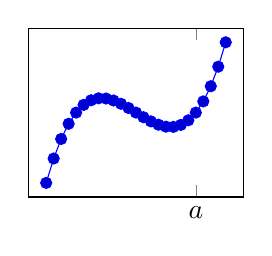
\begin{tikzpicture}
              \begin{axis}[xtick={3}, ytick=\empty, xticklabels={$a$},
                domain=-2:4, width=1.7in]
                \addplot+{(x - 1)*(x+1)*(x-3)+6};
              \end{axis}
            \end{tikzpicture}
            \hspace{0.15in}
            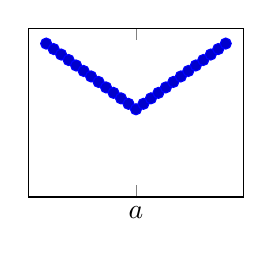
\begin{tikzpicture}
              \begin{axis}[xtick={1}, ytick=\empty, xticklabels={$a$},
                domain=-2:4, width=1.7in, ymin=0]
                \addplot+{abs(x-1) + 4};
              \end{axis}
            \end{tikzpicture}
          \end{center}

        \item $f(x)$ has a \textbf{hole} at $x = a$.  (aka a \textbf{removable discontinuity}.)
          \begin{center}
            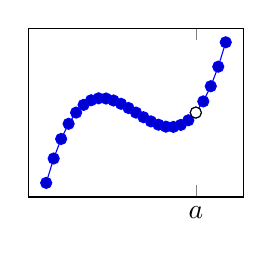
\begin{tikzpicture}
              \begin{axis}[xtick={3}, ytick=\empty, xticklabels={$a$},
                domain=-2:4, width=1.7in]
                \addplot+{(x - 1)*(x+1)*(x-3)+6};
                \addplot[only marks, mark=*, fill=white]
                coordinates { (3, 6) };
              \end{axis}
            \end{tikzpicture}
            \hspace{0.15in}
            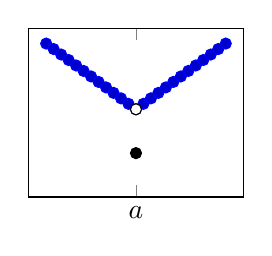
\begin{tikzpicture}
              \begin{axis}[xtick={1}, ytick=\empty, xticklabels={$a$},
                domain=-2:4, width=1.7in, ymin=0]
                \addplot+{abs(x-1) + 4};
                \addplot[only marks, mark=*, fill=white]
                coordinates { (1, 4) }; 
                \addplot[only marks, mark=*, fill=black]
                coordinates { (1, 2) }; 
              \end{axis}
            \end{tikzpicture}
          \end{center}

        \item $f(x)$ has a \textbf{jump discontinuity} at $x = a$.
          \begin{center}
            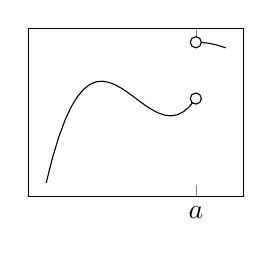
\begin{tikzpicture}
              \begin{axis}[xtick={3}, ytick=\empty, xticklabels={$a$},
                domain=-2:4, width=1.7in, cycle list=black]
                \addplot+[domain=-2:3]{(x - 1)*(x+1)*(x-3)+6};
                \addplot+[domain=3:4] {16-(x-3)^2};
                \addplot[only marks, mark=*, fill=white]
                coordinates { (3, 6) (3, 16)};
              \end{axis}
            \end{tikzpicture}
            \hspace{0.15in}
            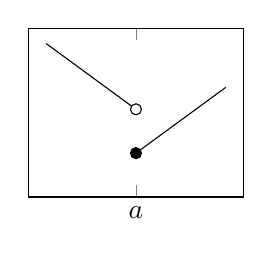
\begin{tikzpicture}
              \begin{axis}[xtick={1}, ytick=\empty, xticklabels={$a$},
                domain=-2:4, width=1.7in, ymin=0, cycle list=black]
                \addplot+[domain=-2:1]{abs(x-1) + 4};
                \addplot+[domain=1:4] {x + 1};
                \addplot[only marks, mark=*, fill=white]
                coordinates { (1, 4) }; 
                \addplot[only marks, mark=*, fill=black]
                coordinates { (1, 2) }; 
              \end{axis}
            \end{tikzpicture}
          \end{center}

        \item $f(x)$ has a \textbf{vertical asymptote} at $x = a$.
          \begin{center}
            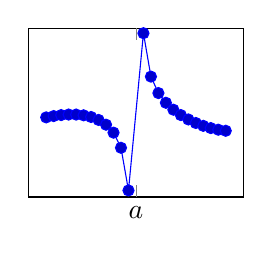
\begin{tikzpicture}
              \begin{axis}[xtick=\empty, extra x ticks={1}, ytick=\empty,
                extra x tick labels={$a$}, domain=-2:4, width=1.7in,
                ymin=-2, ymax=5]
                \addplot+{ sin(deg(x))/(x-1)+1};
              \end{axis}
            \end{tikzpicture}
            \hspace{0.15in}
            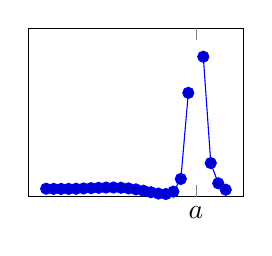
\begin{tikzpicture}
              \begin{axis}[xtick=\empty, extra x ticks={3}, ytick=\empty,
                extra x tick labels={$a$},
                domain=-2:4, width=1.7in, ymin=0, ymax=20,
                restrict y to domain=0:20]
                \addplot+{cos(2*deg(x))/(x-3)^2 + 1};
              \end{axis}
            \end{tikzpicture}
          \end{center}          
        \end{enumerate}

      \end{multicols}      
    \end{minipage}

  \pspace{\newpage}
  
  % \item
  %   \begin{problem}[\stretch{3}]
  %     Let $f(x) = \dfrac{\sin (x^2 - 4)}{x^2 - 4}$.  For what values of
  %     $x$ is $f(x)$ NOT defined?  At each such value, does $f$ have a
  %     removable discontinuity, a jump, or a vertical asymptote?  Use
  %     limits to support your answers (write down each limit you're
  %     calculating, how you calculate it, and what you conclude from it).
  %   \end{problem}

  %   \begin{solution}
  %     The only thing that would cause $f$ to be undefined is the
  %     denominator being 0, which happens when $x = \pm 2$.

  %     Let's look first at $x = 2$.  To decide what type of discontinuity
  %     occurs there, we should calculate $\displaystyle \lim_{x \to 2}
  %     f(x)$, which is a $\frac{0}{0}$ limit:
  %     \begin{align*}
  %       \lim_{x \to 2} \frac{\sin(x^2 - 4)}{x^2 - 4} & \lheq
  %       \lim_{x \to 2} \frac{\cos(x^2 - 4) \cdot 2x}{2x} \\
  %       & \nolheq \lim_{x \to 2} \cos(x^2 - 4) \\
  %       & \nolheq 1
  %     \end{align*}
  %     Since $\displaystyle \lim_{x \to 2} f(x)$ exists, $f$ has a
  %     removable discontinuity (or hole) at $x = 2$.

  %     Notice that $f$ is an even function (because $f(-x) = f(x)$), so $f$
  %     must also have a hole at $x = -2$.

  %     So, $f$ has \fbox{removable discontinuities at $x = \pm 2$}.
  %   \end{solution}


\item 

\begin{grading}
20 points, as follows: 4/4/4/2/2/4
\end{grading}

Let $f(x) = x e^{1/x}$.  
  \begin{enumerate}

  \item
    \begin{problem}[\vfill]
      Find all $x$-values $a$ for which $f(a)$ is undefined.  
      For each value, evaluate $\displaystyle \lim_{x \to a^-} f(x)$ and
      $\displaystyle \lim_{x \to a^+} f(x)$. 
    \end{problem}

    \begin{solution}
      The only value of $x$ for which $x e^{1/x}$ is undefined is $x
        = 0$ (since then $\frac{1}{x}$ is undefined).

      As $x \to 0^-$, $\frac{1}{x} \to - \infty$, so $e^{1/x} \to 0$.
      Therefore, $\displaystyle \lim_{x \to 0^-} x e^{1/x} = 0$.

      As $x \to 0^+$, $\frac{1}{x} \to \infty$, so $e^{1/x} \to \infty$.
      Therefore, $\displaystyle \lim_{x \to 0^+} x e^{1/x}$ is a $0 \cdot
      \infty$ limit, and we should rewrite it so that we can use
      L'Hôpital's Rule:
      \begin{align*}
        \lim_{x \to 0^+} x e^{1/x} & \nolheq \lim_{x \to 0^+}
        \frac{e^{1/x}}{x^{-1}} \\
        & \lheq \lim_{x \to 0^+} \frac{e^{1/x} \left( - x^{-2}
          \right)}{-x^{-2}} \\
        & \nolheq \lim_{x \to 0^+} e^{1/x} \\
        & \nolheq \infty
      \end{align*}
      So, to summarize, $\boxed{\lim_{x \to 0^-} x e^{1/x} = 0}$ and
      $\boxed{ \lim_{x \to 0^+} x e^{1/x} = \infty}$. 
    \end{solution}

  \item
    \begin{problem}[\vfill]
      Find all horizontal asymptotes by calculating the relevant
      limits. 
    \end{problem}

    \begin{solution}
      We need to calculate $\displaystyle \lim_{x \to \infty} f(x)$ and
      $\displaystyle \lim_{x \to -\infty} f(x)$.

      As $x \to \infty$, $\frac{1}{x} \to 0$, so $e^{1/x} \to e^0 = 1$.
      Therefore, $\boxed{\ \lim_{x \to \infty} x e^{1/x} = \infty}$.

      Similarly, as $x \to -\infty$, $\frac{1}{x} \to 0$, so $e^{1/x} \to
      e^0 = 1$, so $\boxed{ \lim_{x \to -\infty} x e^{1/x} = - \infty}$.

      Therefore, $f$ has \fbox{no horizontal asymptotes}. 
    \end{solution}

  \item
    \begin{problem}[\stretch{2}]
      For what values of $x$ is $f(x)$ increasing? 
    \end{problem}

    \begin{solution}
      Let's make a sign chart for $f'$ to answer this.  First, we
      calculate $f'$:
      \begin{align*}
        f'(x) = {} & \frac{d}{dx}
        \left(\fcolorbox{green}{white}{$\displaystyle  x$}\cdot
          \fcolorbox{green}{white}{$\displaystyle  e^ { 1/x } $}\right) \\
        = {} & x\cdot \frac{d}{dx} \left(\fcolorbox{red}{white}{$\displaystyle e^ { \fcolorbox{blue}{white}{$\displaystyle 1/x $}} $}\right)+ e^ { 1/x } \\
        = {} & x\cdot \left(e^ { 1/x } \cdot -x^ { -2} \right)+ e^ { 1/x }
        \\
        = {} & e^{1/x} \left( - \frac{1}{x} + 1 \right)
      \end{align*}
      This is undefined when $x = 0$, and it's 0 when either $e^{1/x} = 0$
      (which never happens) or when $- \frac{1}{x} + 1 = 0$ (which happens
      when $x = 1$).  Testing points, we get the following sign chart for
      $f'$:
      \begin{center}
        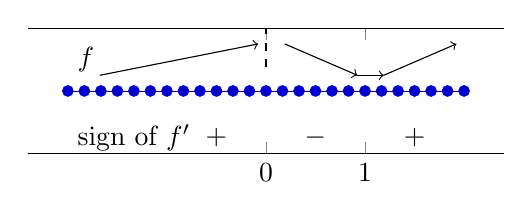
\begin{tikzpicture}
          \begin{axis}[axis y line=none, x axis line style={-}, xtick={0., 1.}, xticklabels={$0$, $1$}, ymin=-2, ymax=2, height=1.25in, width=3in]
            \addplot+[domain=-2.:2., very thin]{0};
            \draw (axis cs: -2., -1.5) node[right] {sign of $f'$};
            \draw (axis cs: -2., 1) node[right] {$f$};
            \draw (axis cs: -0.5, -1.5) node{$+$};
            \draw[->, xshift=2pt] (axis cs: -1.73333, 0.5) -- (axis cs: -0.133333, 1.5);
            \draw (axis cs: 0.5, -1.5) node{$-$};
            \draw[->, xshift=2pt] (axis cs: 0.133333, 1.5) -- (axis cs: 0.866667, 0.5);
            \draw (axis cs: 1.5, -1.5) node{$+$};
            \draw[->, xshift=2pt] (axis cs: 1.13333, 0.5) -- (axis cs: 1.86667, 1.5);
            \draw[dashed] (axis cs: 0, 0.75) -- (axis cs: 0, 2); 
            \draw[->, xshift=2pt] (axis cs: 0.866667, 0.5) -- (axis cs: 1.13333, 0.5);
          \end{axis}
        \end{tikzpicture}        
      \end{center}
      Remember that $f$ has a discontinuity at $x=0$. So, even though this is NOT a critical point (since $x=0$ is not in the domain of $f$), we must stop and
      restart our sign chart there.

Therefore, $f(x)$ is increasing on the intervals $\boxed{(-\infty,0)}$ and $\boxed{(1, \infty)}$.
    \end{solution}

    \pspace{\newpage}

  \item
    \begin{problem}[\vfill]
      List all local extrema of $f$ (on its domain).  Please give the $x$-
      and $y$-coordinates of each local extremum, and say whether it's a
      local minimum or local maximum. 
    \end{problem}

    \begin{solution}
      From our sign chart for $f'$, we can see that the only local
      extremum is a local minimum at $x = 1$, and the corresponding
      $y$-value is $f(1) = e$. 
    \end{solution}

  \item
    \begin{problem}[\vfill]
      Find $\displaystyle \lim_{x \to \infty} f'(x)$ and $\displaystyle
      \lim_{x \to - \infty} f'(x)$.
    \end{problem}

    \begin{solution}
      We already found that $f'(x) = e^{1/x} \left( - \frac{1}{x} + 1
      \right)$.  As $x \to \pm \infty$, $\frac{1}{x} \to 0$, so
      $\displaystyle e^{1/x} \left( - \frac{1}{x} + 1 \right) \to e^0
      \left( 0 + 1 \right) = 1$.  Thus, \fbox{both limits are $1$}.
    \end{solution}

  \item
    \begin{problem}[\stretch{2}]
      Sketch a graph of $f(x)$.  (You need not show the
      concavity accurately, but your graph should accurately reflect what
      you've done in the earlier parts of this problem.)
    \end{problem}

    \begin{solution}
      \begin{center}
        \begin{tikzpicture}
          \begin{axis}[xtick={1}, ymin=-10, ymax=10, ytick={2.72},
            yticklabels={$e$}, axis equal=true, width=3in, height=3in,
            cycle list=black] 
            \addplot+[domain=-10:-0.01, samples=51] { x * e^(1/x)};            
            \addplot+[domain=0.25:10, samples=51] {x * e^(1/x)};
            \addplot[only marks, mark=*, fill=white] coordinates
            { (0, 0) };
          \end{axis}
        \end{tikzpicture}
      \end{center}
       \checkmark\ 
        The key features your graph should have are:
        \begin{itemize}
        \item $\displaystyle \lim_{x \to 0^-} f(x) = 0$ and $\displaystyle
          \lim_{x \to 0^+} f(x) = \infty$.
        \item A local minimum at $(1, e)$.
        \item As $x \to \pm \infty$, the graph of $f$ is almost linear
          with a slope of 1. 
        \end{itemize}
    \end{solution}

  \end{enumerate}

  \probonly{\emph{You are encouraged to use a calculator to check your
      graph after you've sketched it by hand.}}

\pspace{\newpage}


\item 

\begin{grading}
5 points. 2 for part (a), and 3 for part (b).
\end{grading}

 \textbf{Reflect Back.} Reginald says, ``I don't understand why
  $1^\infty$ is an indeterminate form.  If I raise $1$ to any large power,
  the answer is 1, so why aren't $1^\infty$ limits just equal to 1?''

  \begin{enumerate}
  \item
    \begin{problem}[\vfill]
      Write a response to Reginald.
    \end{problem}

    \begin{solution}
      When we evaluate a $1^\infty$ limit, we're not necessarily raising
      $1$ to a very large power; it's more accurate to think about raising
      a number very close to 1 to a very large power.  For
        example, when you looked numerically at the limit $\displaystyle
        \lim_{h \to 0^+} (1 + h)^{1/h}$ in {{{Problem Set 17}, {{\#6}}}}, plugging
        in tiny values of $h$ involved raising numbers slightly greater
        than 1 to very large powers.  But this can give a great variety
      of results; for example, raising $0.99$ to a huge power can give a
      tiny answer, while raising $1.01$ to a huge power can give a huge
      answer.
    \end{solution}

  \item
    \begin{problem}
      All of the limits below can be evaluated easily, just by using
      algebra to simplify them.  Three of them are of the form $1^\infty$;
      identify those three and evaluate them, as another way to convince
      Reginald that $1^\infty$ really is an indeterminate form.
    \end{problem}

    
      \begin{enumerate}[label=\protect\maybecircle{\Alph*.}]
      \plainitem $\displaystyle \lim_{x \to \infty} \left(2^x
        \right)^{1/x}$
      \plainitem $\displaystyle \lim_{x \to -\infty} \left( e^x
        \right)^{-1/x}$
      \circleitem $\displaystyle \lim_{x \to \infty} 1^x$
      \plainitem $\displaystyle \lim_{x \to \infty} \left( 5^x
        \right)^{-1/x}$ 
      \circleitem $\displaystyle \lim_{x \to 0^+} \left( 3^x
        \right)^{1/x}$
      \circleitem $\displaystyle \lim_{x \to \infty} \left( e^{1/x}
        \right)^{x^2}$
      \end{enumerate}
    

    \begin{solution}
      $\displaystyle \lim_{x \to \infty} 1^x = 1$ (because $1^x = 1$ for
      all $x$), $\displaystyle \lim_{x \to 0^+} \left( 3^x \right)^{1/x} =
      \lim_{x \to 0^+} 3^{x (1/x)} = 3$, and $\displaystyle \lim_{x \to
        \infty} \left( e^{1/x} \right)^{x^2} = \lim_{x \to \infty} e^x =
      \infty$.
    \end{solution}
  \end{enumerate}  

\pspace{\stretch{2}}

% \pspace{\newpage}
% \item 
% \begin{problem}
%     Midterm 1 scores were released on Wednesday, and a goal of Math Mb this semester is to help you to learn to study for understanding and retention
% in the process of preparing for assessments. Complete the linked Exam Reflection, which is designed to give you a chance to reflect on your exam, your experiences in section and working on PSETs, and on the effectiveness of your exam preparation.
% Please answer the questions sincerely. This will be graded for completion, so your answers in no way affect your grade. Your
% responses will inform the teaching team about students’ experience surrounding the first midterm exam and how we can best support your learning. Your responses here can be used to inform and guide your preparation for Midterm 2 and the final exam.

% You can access the Exam Reflection by clicking \href{https://docs.google.com/forms/d/e/1FAIpQLSeJG8Z99g8vBarLNQKSbfVsonBi9LNVj_ySgtOIaQ_Zzs-U8Q/viewform?usp=sf_link}{\textbf{\textcolor{blue}{here.}}} For your completion to be registered, you must enter your @college.harvard.edu email in the Form.
% \end{problem}

\end{enumerate}

\spaceonly{\psreflection{For next class, read Gottlieb \S 22.1.}}

\end{document}P